\section{تحلیل مدار 
\lr{c17}
}
در این قسمت قصد داریم به تحلیل مدار c17 بپردازیم. ابتدا مدار را به وسیله دو ورودی که حاوی چهار منطق است، بررسی کرده و شبیه سازی 
\lr{true-value}
را انجام می دهیم. در ادامه مدار را به وسیله دو ورودی که حاوی دو منطق است، بررسی می کنیم و شبیه سازی اشکال استنتاجی یا 
\lr{Deductive}
را انجام می دهیم.

\subsection{شبیه سازی 
\lr{true-value}}
شبیه سازی true-value به این صورت است که زمانی شبکه مدار های منطقی شکل گرفت، از لایه صفر یعنی پایانه های ورودی، مقادیر را به مدار تزریق کنیم و خروجی هر گیت را محاسبه و بر روی سیم خروجی گیت قرار دهیم و این روند را از تا زمانی به پیانه های خروجی نرسیده ایم، انجام دهیم.


\begin{figure}[H]
	\begin{center}
		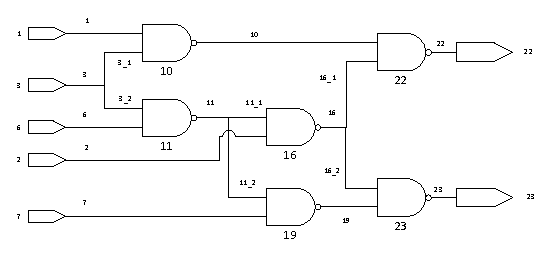
\includegraphics[width=0.8\textwidth]{c17_results/pictures/c17.eps}
	\end{center}
	\caption{
		نمای مدار منطقی مربوط به فایل 
		\lr{c17}
		پس از خواندن فایل به همراه سیم های متصل کننده
	}
	\label{fig:c17}
\end{figure}


\subsubsection{تلاش اول}
در اولین ورودی که قصد داریم به مدار 
\lr{c17}
 اعمال کنیم به شکل زیر است:

\lr{$$1: Z, 3: 0, 6: 1, 2: U , 7: 0$$}

که این ورودی پس از اعمال بر روی شبکه ، خروجی های هر سیم و همچنین خروجی های نهایی، به شکل زیر خواهد بود:

\begin{latin}
\begin{lstlisting}[numbers=left, breaklines=true]
Wire:1, Value:Z 
Wire:2, Value:U 
Wire:3, Value:0 
Wire:6, Value:1 
Wire:7, Value:0 
Wire:3_1, Value:0 
Wire:3_2, Value:0 
Wire:10, Value:1 
Wire:11, Value:1 
Wire:11_1, Value:1 
Wire:11_2, Value:1 
Wire:16, Value:U 
Wire:19, Value:1 
Wire:16_1, Value:U 
Wire:16_2, Value:U 
Wire:22, Value:U 
Wire:23, Value:U 
------------------
Output Gate:22, Value:U 
Output Gate:23, Value:U 
\end{lstlisting}
\end{latin}

\subsubsection{تلاش دوم}
در دومین ورودی که قصد داریم به مدار 
\lr{c17}
اعمال کنیم به شکل زیر است:

\lr{$$1: 0, 3: 1, 6: Z, 2: 1 , 7: U$$}

که این ورودی پس از اعمال بر روی شبکه ، خروجی های هر سیم و همچنین خروجی های نهایی، به شکل زیر خواهد بود:

\begin{latin}
\begin{lstlisting}[numbers=left, breaklines=true]
Wire:1, Value:0 
Wire:2, Value:1 
Wire:3, Value:1 
Wire:6, Value:Z 
Wire:7, Value:U 
Wire:3_1, Value:1 
Wire:3_2, Value:1 
Wire:10, Value:1 
Wire:11, Value:Z 
Wire:11_1, Value:Z 
Wire:11_2, Value:Z 
Wire:16, Value:Z 
Wire:19, Value:U 
Wire:16_1, Value:Z 
Wire:16_2, Value:Z 
Wire:22, Value:Z 
Wire:23, Value:U 
------------------
Output Gate:22, Value:Z 
Output Gate:23, Value:U 
\end{lstlisting}
\end{latin}

\subsection{شبیه سازی اشکال 
\lr{Deductive}}
الگوریتم و کد الگوریتم شبیه سازی اشکال 
\lr{Deductive}
در قسمت های قبلی ، توضیح داده شد. در این قسمت قصد داریم که دو ورودی تست ،‌ با منطق دو مقداره به مدار اعمال کنیم و اشکالات هر سیم و همچنین اشکالاتی که در خروجی نمایان می شوند را مشاهده کنیم.

\subsubsection{تلاش اول}
در اولین بردار تستی که قصد داریم که به مدار 
\lr{c17}
اعمال کنیم، به شکل زیر است: 

\lr{$$1: 1, 3: 0, 6: 1, 2: 0 , 7: 0$$}

که این بردار تست پس از اعمال بر روی شبکه، اشکالات هر سیم و همچنین اشکالاتی که در خروجی نهایی نمایان می شود، به شکل زیر خواهد بود:

\begin{latin}
\begin{lstlisting}[numbers=left, breaklines=true]
Wire:1, Value:1, Discovered faults:{'1_s-a-0'} 
Wire:2, Value:0, Discovered faults:{'2_s-a-1'} 
Wire:3, Value:0, Discovered faults:{'3_s-a-1'} 
Wire:6, Value:1, Discovered faults:{'6_s-a-0'} 
Wire:7, Value:0, Discovered faults:{'7_s-a-1'} 
Wire:3_1, Value:0, Discovered faults:{'3_s-a-1', '3_1_s-a-1'} 
Wire:3_2, Value:0, Discovered faults:{'3_s-a-1', '3_2_s-a-1'} 
Wire:10, Value:1, Discovered faults:{'3_s-a-1', '10_s-a-0', '3_1_s-a-1'} 
Wire:11, Value:1, Discovered faults:{'3_s-a-1', '11_s-a-0', '3_2_s-a-1'} 
Wire:11_1, Value:1, Discovered faults:{'3_s-a-1', '11_s-a-0', '11_1_s-a-0', '3_2_s-a-1'} 
Wire:11_2, Value:1, Discovered faults:{'3_s-a-1', '11_s-a-0', '11_2_s-a-0', '3_2_s-a-1'} 
Wire:16, Value:1, Discovered faults:{'16_s-a-0', '2_s-a-1'} 
Wire:19, Value:1, Discovered faults:{'19_s-a-0', '7_s-a-1'} 
Wire:16_1, Value:1, Discovered faults:{'16_s-a-0', '2_s-a-1', '16_1_s-a-0'} 
Wire:16_2, Value:1, Discovered faults:{'16_s-a-0', '2_s-a-1', '16_2_s-a-0'} 
Wire:22, Value:0, Discovered faults:{'10_s-a-0', '16_s-a-0', '2_s-a-1', '16_1_s-a-0', '22_s-a-1', '3_1_s-a-1', '3_s-a-1'} 
Wire:23, Value:0, Discovered faults:{'16_s-a-0', '2_s-a-1', '16_2_s-a-0', '19_s-a-0', '23_s-a-1', '7_s-a-1'} 
------------------
OutputGate: 22, Value:0, Wire:22, Discoverd faults:{'10_s-a-0', '16_s-a-0', '2_s-a-1', '16_1_s-a-0', '22_s-a-1', '3_1_s-a-1', '3_s-a-1'} 
OutputGate: 23, Value:0, Wire:23, Discoverd faults:{'16_s-a-0', '2_s-a-1', '16_2_s-a-0', '19_s-a-0', '23_s-a-1', '7_s-a-1'} 
\end{lstlisting}
\end{latin}

\subsubsection{تلاش دوم}

در دومین بردار تستی که قصد داریم که به مدار 
\lr{c17}
اعمال کنیم، به شکل زیر است: 

\lr{$$1: 1, 3: 0, 6: 0, 2: 1 , 7: 1$$}

\begin{latin}
\begin{lstlisting}[numbers=left, breaklines=true]
Wire:1, Value:1, Discovered faults:{'1_s-a-0'} 
Wire:2, Value:1, Discovered faults:{'2_s-a-0'} 
Wire:3, Value:0, Discovered faults:{'3_s-a-1'} 
Wire:6, Value:0, Discovered faults:{'6_s-a-1'} 
Wire:7, Value:1, Discovered faults:{'7_s-a-0'} 
Wire:3_1, Value:0, Discovered faults:{'3_1_s-a-1', '3_s-a-1'} 
Wire:3_2, Value:0, Discovered faults:{'3_2_s-a-1', '3_s-a-1'} 
Wire:10, Value:1, Discovered faults:{'3_1_s-a-1', '3_s-a-1', '10_s-a-0'} 
Wire:11, Value:1, Discovered faults:{'11_s-a-0'} 
Wire:11_1, Value:1, Discovered faults:{'11_1_s-a-0', '11_s-a-0'} 
Wire:11_2, Value:1, Discovered faults:{'11_2_s-a-0', '11_s-a-0'} 
Wire:16, Value:0, Discovered faults:{'11_1_s-a-0', '16_s-a-1', '2_s-a-0', '11_s-a-0'} 
Wire:19, Value:0, Discovered faults:{'11_2_s-a-0', '19_s-a-1', '11_s-a-0', '7_s-a-0'} 
Wire:16_1, Value:0, Discovered faults:{'2_s-a-0', '11_s-a-0', '11_1_s-a-0', '16_s-a-1', '16_1_s-a-1'} 
Wire:16_2, Value:0, Discovered faults:{'2_s-a-0', '11_s-a-0', '16_2_s-a-1', '11_1_s-a-0', '16_s-a-1'} 
Wire:22, Value:1, Discovered faults:{'22_s-a-0', '2_s-a-0', '11_1_s-a-0', '16_s-a-1', '16_1_s-a-1', '11_s-a-0'} 
Wire:23, Value:1, Discovered faults:{'23_s-a-0', '11_s-a-0'} 
------------------
OutputGate: 22, Value:1, Wire:22, Discoverd faults:{'22_s-a-0', '2_s-a-0', '11_1_s-a-0', '16_s-a-1', '16_1_s-a-1', '11_s-a-0'} 
OutputGate: 23, Value:1, Wire:23, Discoverd faults:{'23_s-a-0', '11_s-a-0'} 
\end{lstlisting}
\end{latin}

